%% figures/fig-phase.tex -- Figure for Sec. 4.4.
%% Pulled into notes.tex with %% figures/fig-phase.tex -- Figure for Sec. 4.4.
%% Pulled into notes.tex with %% figures/fig-phase.tex -- Figure for Sec. 4.4.
%% Pulled into notes.tex with %% figures/fig-phase.tex -- Figure for Sec. 4.4.
%% Pulled into notes.tex with \input{figures/fig-phase}.
%% Needs pgfplots, loaded in the main preamble.
%%
%% Plots a(v) = [ -(3/8k) ln((1+v)/(1-v)) + C ] (1-v^2)^{3/2}, the closed-form
%% phase portrait of branch (a). Nothing here is drawn by hand: the zeros
%% marked on the v axis are v* = tanh(4 k C / 3), which follows from setting
%% the bracket to zero, and for the two curves shown they are
%%
%%   k = 1/2, C = 1  ->  v* = tanh(2/3)  = 0.5827
%%   k = 1,   C = 1  ->  v* = tanh(4/3)  = 0.8701
%%
%% Only v > 0 is drawn; the portrait is symmetric under (v,a,C) -> (-v,-a,-C).

\begin{figure}[htb]
\centering
\begin{tikzpicture}
\begin{axis}[
  width=12.2cm, height=8.1cm,
  xlabel={$v$}, ylabel={$a$},
  xmin=0, xmax=1.02, ymin=-0.62, ymax=1.30,
  axis lines=middle,
  xtick={0.2,0.4,0.6,0.8,1.0},
  xticklabel style={anchor=north,yshift=-1pt},
  ytick=\empty,
  every axis y label/.style={at={(ticklabel* cs:1.0)},anchor=south east},
  every axis x label/.style={at={(ticklabel* cs:1.0)},anchor=north west},
  clip=true, samples=200, font=\footnotesize,
]

  %% drop lines marking the two equilibria, drawn first so the curves sit on top
  \draw[gray,dashed] (axis cs:0.5827,0) -- (axis cs:0.5827,-0.30);
  \draw[gray,dashed] (axis cs:0.8701,0) -- (axis cs:0.8701,-0.30);
  \node[anchor=north,font=\footnotesize] at (axis cs:0.5827,-0.30)
       {$v_*=\tanh\tfrac23$};
  \node[anchor=north,font=\footnotesize] at (axis cs:0.8701,-0.30)
       {$\tanh\tfrac43$};

  %% kappa < 0 : the Lorentz-Dirac value. a stays above the axis.
  \addplot[very thick,domain=0:0.995]
      {( 0.75*ln((1+x)/(1-x)) + 1 ) * (1-x^2)^(3/2)};
  \node[align=center,font=\footnotesize] at (axis cs:0.50,0.80)
       {$\kappa=-\tfrac12$\\(Lorentz--Dirac)};

  %% kappa > 0 : crosses the axis and returns to it
  \addplot[thick,domain=0:0.995]
      {( -0.375*ln((1+x)/(1-x)) + 1 ) * (1-x^2)^(3/2)};
  \node[anchor=south west,font=\footnotesize] at (axis cs:0.63,0.20)
       {$\kappa=+1$};

  \addplot[thick,domain=0:0.995]
      {( -0.75*ln((1+x)/(1-x)) + 1 ) * (1-x^2)^(3/2)};
  \node[anchor=south west,font=\footnotesize] at (axis cs:0.135,0.44)
       {$\kappa=+\tfrac12$};

  %% the equilibria themselves
  \fill (axis cs:0.5827,0) circle (1.6pt);
  \fill (axis cs:0.8701,0) circle (1.6pt);

\end{axis}
\end{tikzpicture}
\caption{The phase portrait of branch (a), Eq.~(\ref{eq:phase}), for $C=1$. The sign of $\kappa$ decides everything. For $\kappa<0$,
which includes the Lorentz--Dirac value $\kappa=-\tfrac12$, the bracket grows
with $v$ and the curve never returns to the axis: the acceleration is positive
at every speed, so nothing stops the particle short of $c$, and this is the
runaway of Sec.~\ref{sec:freesol} seen in the $(v,a)$ plane. For $\kappa>0$ the
bracket decreases, the curve must cross the axis, and the crossing at
$v_*=\tanh(4\kappa C/3)$ is an attractor: below it the acceleration is positive
and above it negative, so a particle released anywhere returns to $v_*$. The
terminal speed is then fixed by $C$, which is fixed by the applied impulse ---
force determines velocity rather than acceleration, which is why
\citet{zhang2006} calls this Aristotle motion. Only $v>0$ is shown; the
portrait is symmetric under $(v,a,C)\to(-v,-a,-C)$.
\label{fig:phase}}
\end{figure}
.
%% Needs pgfplots, loaded in the main preamble.
%%
%% Plots a(v) = [ -(3/8k) ln((1+v)/(1-v)) + C ] (1-v^2)^{3/2}, the closed-form
%% phase portrait of branch (a). Nothing here is drawn by hand: the zeros
%% marked on the v axis are v* = tanh(4 k C / 3), which follows from setting
%% the bracket to zero, and for the two curves shown they are
%%
%%   k = 1/2, C = 1  ->  v* = tanh(2/3)  = 0.5827
%%   k = 1,   C = 1  ->  v* = tanh(4/3)  = 0.8701
%%
%% Only v > 0 is drawn; the portrait is symmetric under (v,a,C) -> (-v,-a,-C).

\begin{figure}[htb]
\centering
\begin{tikzpicture}
\begin{axis}[
  width=12.2cm, height=8.1cm,
  xlabel={$v$}, ylabel={$a$},
  xmin=0, xmax=1.02, ymin=-0.62, ymax=1.30,
  axis lines=middle,
  xtick={0.2,0.4,0.6,0.8,1.0},
  xticklabel style={anchor=north,yshift=-1pt},
  ytick=\empty,
  every axis y label/.style={at={(ticklabel* cs:1.0)},anchor=south east},
  every axis x label/.style={at={(ticklabel* cs:1.0)},anchor=north west},
  clip=true, samples=200, font=\footnotesize,
]

  %% drop lines marking the two equilibria, drawn first so the curves sit on top
  \draw[gray,dashed] (axis cs:0.5827,0) -- (axis cs:0.5827,-0.30);
  \draw[gray,dashed] (axis cs:0.8701,0) -- (axis cs:0.8701,-0.30);
  \node[anchor=north,font=\footnotesize] at (axis cs:0.5827,-0.30)
       {$v_*=\tanh\tfrac23$};
  \node[anchor=north,font=\footnotesize] at (axis cs:0.8701,-0.30)
       {$\tanh\tfrac43$};

  %% kappa < 0 : the Lorentz-Dirac value. a stays above the axis.
  \addplot[very thick,domain=0:0.995]
      {( 0.75*ln((1+x)/(1-x)) + 1 ) * (1-x^2)^(3/2)};
  \node[align=center,font=\footnotesize] at (axis cs:0.50,0.80)
       {$\kappa=-\tfrac12$\\(Lorentz--Dirac)};

  %% kappa > 0 : crosses the axis and returns to it
  \addplot[thick,domain=0:0.995]
      {( -0.375*ln((1+x)/(1-x)) + 1 ) * (1-x^2)^(3/2)};
  \node[anchor=south west,font=\footnotesize] at (axis cs:0.63,0.20)
       {$\kappa=+1$};

  \addplot[thick,domain=0:0.995]
      {( -0.75*ln((1+x)/(1-x)) + 1 ) * (1-x^2)^(3/2)};
  \node[anchor=south west,font=\footnotesize] at (axis cs:0.135,0.44)
       {$\kappa=+\tfrac12$};

  %% the equilibria themselves
  \fill (axis cs:0.5827,0) circle (1.6pt);
  \fill (axis cs:0.8701,0) circle (1.6pt);

\end{axis}
\end{tikzpicture}
\caption{The phase portrait of branch (a), Eq.~(\ref{eq:phase}), for $C=1$. The sign of $\kappa$ decides everything. For $\kappa<0$,
which includes the Lorentz--Dirac value $\kappa=-\tfrac12$, the bracket grows
with $v$ and the curve never returns to the axis: the acceleration is positive
at every speed, so nothing stops the particle short of $c$, and this is the
runaway of Sec.~\ref{sec:freesol} seen in the $(v,a)$ plane. For $\kappa>0$ the
bracket decreases, the curve must cross the axis, and the crossing at
$v_*=\tanh(4\kappa C/3)$ is an attractor: below it the acceleration is positive
and above it negative, so a particle released anywhere returns to $v_*$. The
terminal speed is then fixed by $C$, which is fixed by the applied impulse ---
force determines velocity rather than acceleration, which is why
\citet{zhang2006} calls this Aristotle motion. Only $v>0$ is shown; the
portrait is symmetric under $(v,a,C)\to(-v,-a,-C)$.
\label{fig:phase}}
\end{figure}
.
%% Needs pgfplots, loaded in the main preamble.
%%
%% Plots a(v) = [ -(3/8k) ln((1+v)/(1-v)) + C ] (1-v^2)^{3/2}, the closed-form
%% phase portrait of branch (a). Nothing here is drawn by hand: the zeros
%% marked on the v axis are v* = tanh(4 k C / 3), which follows from setting
%% the bracket to zero, and for the two curves shown they are
%%
%%   k = 1/2, C = 1  ->  v* = tanh(2/3)  = 0.5827
%%   k = 1,   C = 1  ->  v* = tanh(4/3)  = 0.8701
%%
%% Only v > 0 is drawn; the portrait is symmetric under (v,a,C) -> (-v,-a,-C).

\begin{figure}[htb]
\centering
\begin{tikzpicture}
\begin{axis}[
  width=12.2cm, height=8.1cm,
  xlabel={$v$}, ylabel={$a$},
  xmin=0, xmax=1.02, ymin=-0.62, ymax=1.30,
  axis lines=middle,
  xtick={0.2,0.4,0.6,0.8,1.0},
  xticklabel style={anchor=north,yshift=-1pt},
  ytick=\empty,
  every axis y label/.style={at={(ticklabel* cs:1.0)},anchor=south east},
  every axis x label/.style={at={(ticklabel* cs:1.0)},anchor=north west},
  clip=true, samples=200, font=\footnotesize,
]

  %% drop lines marking the two equilibria, drawn first so the curves sit on top
  \draw[gray,dashed] (axis cs:0.5827,0) -- (axis cs:0.5827,-0.30);
  \draw[gray,dashed] (axis cs:0.8701,0) -- (axis cs:0.8701,-0.30);
  \node[anchor=north,font=\footnotesize] at (axis cs:0.5827,-0.30)
       {$v_*=\tanh\tfrac23$};
  \node[anchor=north,font=\footnotesize] at (axis cs:0.8701,-0.30)
       {$\tanh\tfrac43$};

  %% kappa < 0 : the Lorentz-Dirac value. a stays above the axis.
  \addplot[very thick,domain=0:0.995]
      {( 0.75*ln((1+x)/(1-x)) + 1 ) * (1-x^2)^(3/2)};
  \node[align=center,font=\footnotesize] at (axis cs:0.50,0.80)
       {$\kappa=-\tfrac12$\\(Lorentz--Dirac)};

  %% kappa > 0 : crosses the axis and returns to it
  \addplot[thick,domain=0:0.995]
      {( -0.375*ln((1+x)/(1-x)) + 1 ) * (1-x^2)^(3/2)};
  \node[anchor=south west,font=\footnotesize] at (axis cs:0.63,0.20)
       {$\kappa=+1$};

  \addplot[thick,domain=0:0.995]
      {( -0.75*ln((1+x)/(1-x)) + 1 ) * (1-x^2)^(3/2)};
  \node[anchor=south west,font=\footnotesize] at (axis cs:0.135,0.44)
       {$\kappa=+\tfrac12$};

  %% the equilibria themselves
  \fill (axis cs:0.5827,0) circle (1.6pt);
  \fill (axis cs:0.8701,0) circle (1.6pt);

\end{axis}
\end{tikzpicture}
\caption{The phase portrait of branch (a), Eq.~(\ref{eq:phase}), for $C=1$. The sign of $\kappa$ decides everything. For $\kappa<0$,
which includes the Lorentz--Dirac value $\kappa=-\tfrac12$, the bracket grows
with $v$ and the curve never returns to the axis: the acceleration is positive
at every speed, so nothing stops the particle short of $c$, and this is the
runaway of Sec.~\ref{sec:freesol} seen in the $(v,a)$ plane. For $\kappa>0$ the
bracket decreases, the curve must cross the axis, and the crossing at
$v_*=\tanh(4\kappa C/3)$ is an attractor: below it the acceleration is positive
and above it negative, so a particle released anywhere returns to $v_*$. The
terminal speed is then fixed by $C$, which is fixed by the applied impulse ---
force determines velocity rather than acceleration, which is why
\citet{zhang2006} calls this Aristotle motion. Only $v>0$ is shown; the
portrait is symmetric under $(v,a,C)\to(-v,-a,-C)$.
\label{fig:phase}}
\end{figure}
.
%% Needs pgfplots, loaded in the main preamble.
%%
%% Plots a(v) = [ -(3/8k) ln((1+v)/(1-v)) + C ] (1-v^2)^{3/2}, the closed-form
%% phase portrait of branch (a). Nothing here is drawn by hand: the zeros
%% marked on the v axis are v* = tanh(4 k C / 3), which follows from setting
%% the bracket to zero, and for the two curves shown they are
%%
%%   k = 1/2, C = 1  ->  v* = tanh(2/3)  = 0.5827
%%   k = 1,   C = 1  ->  v* = tanh(4/3)  = 0.8701
%%
%% Only v > 0 is drawn; the portrait is symmetric under (v,a,C) -> (-v,-a,-C).

\begin{figure}[htb]
\centering
\begin{tikzpicture}
\begin{axis}[
  width=12.2cm, height=8.1cm,
  xlabel={$v$}, ylabel={$a$},
  xmin=0, xmax=1.02, ymin=-0.62, ymax=1.30,
  axis lines=middle,
  xtick={0.2,0.4,0.6,0.8,1.0},
  xticklabel style={anchor=north,yshift=-1pt},
  ytick=\empty,
  every axis y label/.style={at={(ticklabel* cs:1.0)},anchor=south east},
  every axis x label/.style={at={(ticklabel* cs:1.0)},anchor=north west},
  clip=true, samples=200, font=\footnotesize,
]

  %% drop lines marking the two equilibria, drawn first so the curves sit on top
  \draw[gray,dashed] (axis cs:0.5827,0) -- (axis cs:0.5827,-0.30);
  \draw[gray,dashed] (axis cs:0.8701,0) -- (axis cs:0.8701,-0.30);
  \node[anchor=north,font=\footnotesize] at (axis cs:0.5827,-0.30)
       {$v_*=\tanh\tfrac23$};
  \node[anchor=north,font=\footnotesize] at (axis cs:0.8701,-0.30)
       {$\tanh\tfrac43$};

  %% kappa < 0 : the Lorentz-Dirac value. a stays above the axis.
  \addplot[very thick,domain=0:0.995]
      {( 0.75*ln((1+x)/(1-x)) + 1 ) * (1-x^2)^(3/2)};
  \node[align=center,font=\footnotesize] at (axis cs:0.50,0.80)
       {$\kappa=-\tfrac12$\\(Lorentz--Dirac)};

  %% kappa > 0 : crosses the axis and returns to it
  \addplot[thick,domain=0:0.995]
      {( -0.375*ln((1+x)/(1-x)) + 1 ) * (1-x^2)^(3/2)};
  \node[anchor=south west,font=\footnotesize] at (axis cs:0.63,0.20)
       {$\kappa=+1$};

  \addplot[thick,domain=0:0.995]
      {( -0.75*ln((1+x)/(1-x)) + 1 ) * (1-x^2)^(3/2)};
  \node[anchor=south west,font=\footnotesize] at (axis cs:0.135,0.44)
       {$\kappa=+\tfrac12$};

  %% the equilibria themselves
  \fill (axis cs:0.5827,0) circle (1.6pt);
  \fill (axis cs:0.8701,0) circle (1.6pt);

\end{axis}
\end{tikzpicture}
\caption{The phase portrait of branch (a), Eq.~(\ref{eq:phase}), for $C=1$. The sign of $\kappa$ decides everything. For $\kappa<0$,
which includes the Lorentz--Dirac value $\kappa=-\tfrac12$, the bracket grows
with $v$ and the curve never returns to the axis: the acceleration is positive
at every speed, so nothing stops the particle short of $c$, and this is the
runaway of Sec.~\ref{sec:freesol} seen in the $(v,a)$ plane. For $\kappa>0$ the
bracket decreases, the curve must cross the axis, and the crossing at
$v_*=\tanh(4\kappa C/3)$ is an attractor: below it the acceleration is positive
and above it negative, so a particle released anywhere returns to $v_*$. The
terminal speed is then fixed by $C$, which is fixed by the applied impulse ---
force determines velocity rather than acceleration, which is why
\citet{zhang2006} calls this Aristotle motion. Only $v>0$ is shown; the
portrait is symmetric under $(v,a,C)\to(-v,-a,-C)$.
\label{fig:phase}}
\end{figure}
